\section{Accelerometer}

\subsection{Task 6}

The question here is similar to homework3 , the pre-function about calculating $ [Hx  ; hx] $.

The measurement model is $ y_k^a=Q^T(q_k)(g^0+f_k^a)+e_k^a $, in which we assume $ f_k^a = 0 $.Then the $ hx = Q^T(q_k) \cdot g^0 $, $ Hx = \frac{\partial{hx}}{\partial{q_k}} = \frac{dQ(q_k)}{dq} \cdot g^0$. In addition, the updating process is :

\begin{equation}
    \begin{aligned}
        \hat{\mathbf{x}}_{k|k}&=\hat{\mathbf{x}}_{k|k-1}+\mathbf{K}_k\mathbf{v}_k\\
        \mathbf{P}_{k|k}&=\mathbf{P}_{k|k-1}-\mathbf{K}_{k}\mathbf{S}_{k}\mathbf{K}_{k}^{T}\\
        &\text{where}\\
        & Q = Qq(x),
        \mathbf{h}  = Q'\cdot \mathbf(g)^0;\\
&[Q0, \quad Q1, \quad Q2,\quad  Q3] = dQqdq(x);\\
&\mathbf{H} = [Q0'\mathbf(g)^0 \quad Q1'\mathbf(g)^0 \quad Q2'\mathbf(g)^0 \quad Q3'\mathbf(g)^0];\\
        &\mathbf{K}_k=\mathbf{P}_{k|k-1}\mathbf{H}_k^T\mathbf{S}_k^{-1}\\
        &\mathbf{v}_k=\mathbf{y}_k-\mathbf{H}_k\hat{\mathbf{x}}_{k|k-1}\\
        &\mathbf{S}_k=\mathbf{H}_k\mathbf{P}_{k|k-1}\mathbf{H}_k^T+\mathbf{R}_k\nonumber
    \end{aligned}
\end{equation}



The $\hat{\mathbf{x}}_{k|k}$ and $ \mathbf{P}_{k|k}  $ above are the return value of the function \texttt{mu\_g}.

\subsection{Task 7}


\begin{figure}[H]
 \centering
 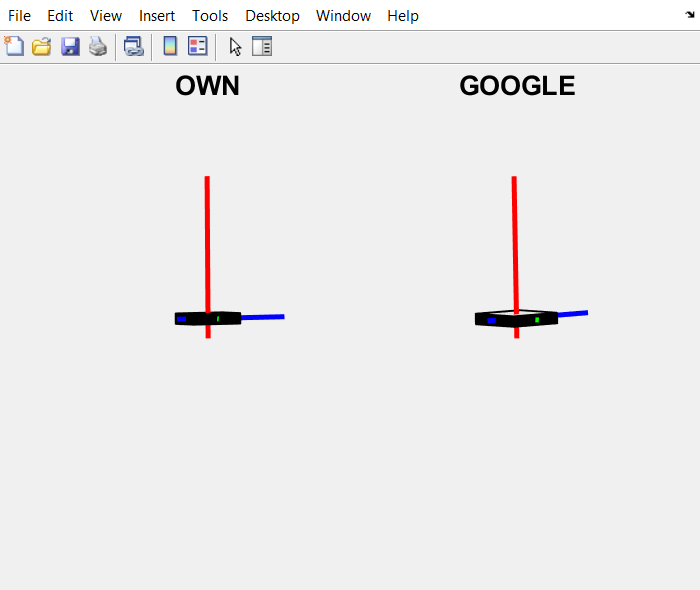
\includegraphics[width=0.6\textwidth]{images/7start.png}
 \caption{Task7 Start figure}
 \label{7start}
\end{figure}

Move the phone right and left at a slow speed repeatedly:

\begin{figure}[H]
 \centering
 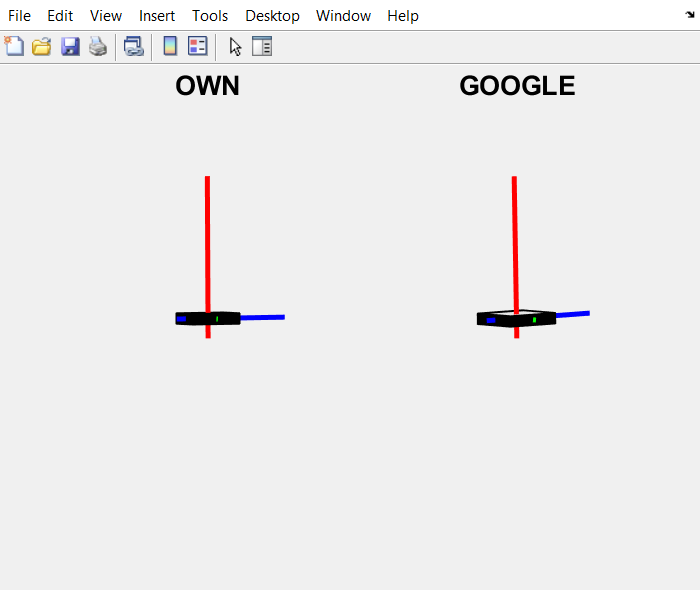
\includegraphics[width=0.6\textwidth]{images/rightleft.png}
 \caption{Right left move }
 \label{rightleft}
\end{figure}

Flip the phone to the right side and lay it down repeatedly:
\begin{figure}[H]
 \centering
 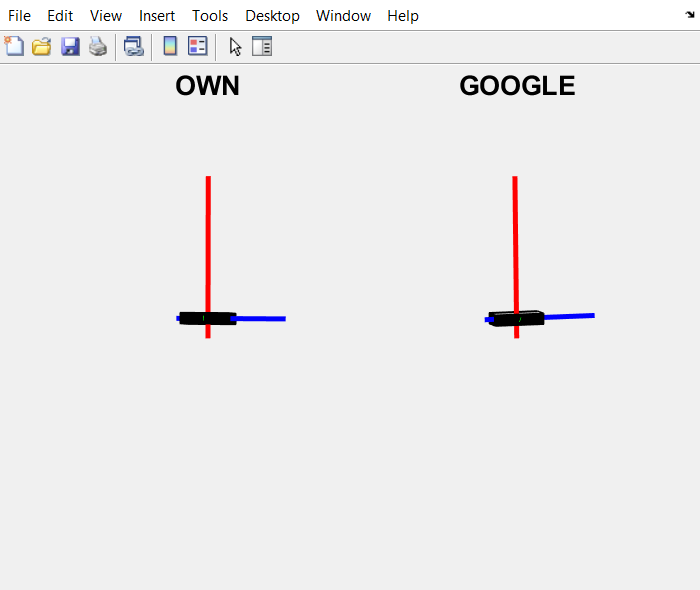
\includegraphics[width=0.6\textwidth]{images/flipright.png}
 \caption{Flip right}
 \label{flipright}
\end{figure}

Fastly flip it forward and back:

\begin{figure}[H]
 \centering
 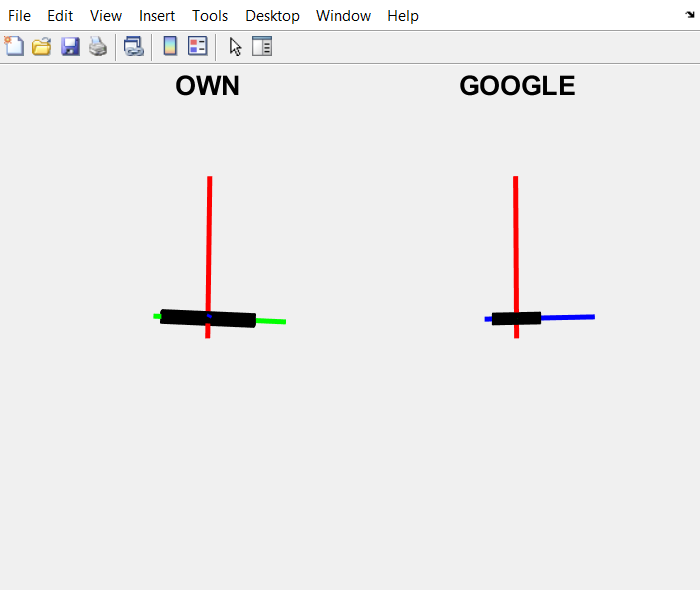
\includegraphics[width=0.6\textwidth]{images/forward.png}
 \caption{Flip forward}
 \label{flipforward}
\end{figure}

Fastly rotate it around $ \mathbf{y} $:

\begin{figure}[H]
 \centering
 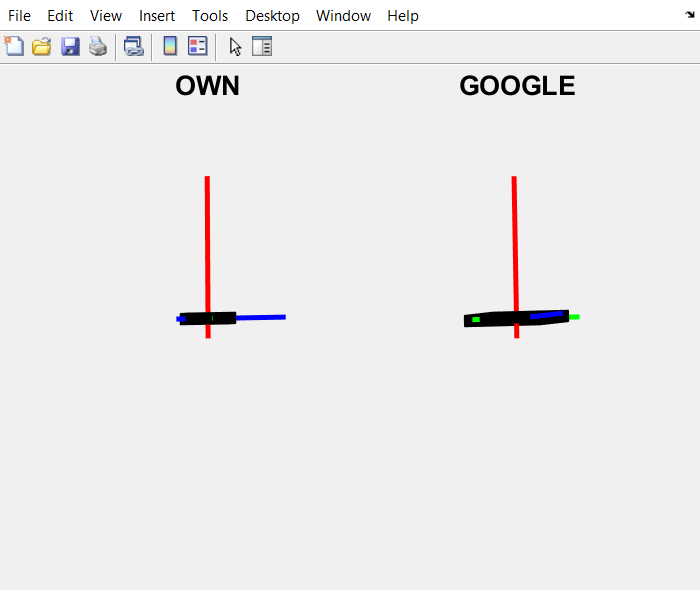
\includegraphics[width=0.6\textwidth]{images/rotatey.png}
 \caption{Rotate around y}
 \label{rotatey}
\end{figure}

Fastly go to right:

\begin{figure}[H]
 \centering
 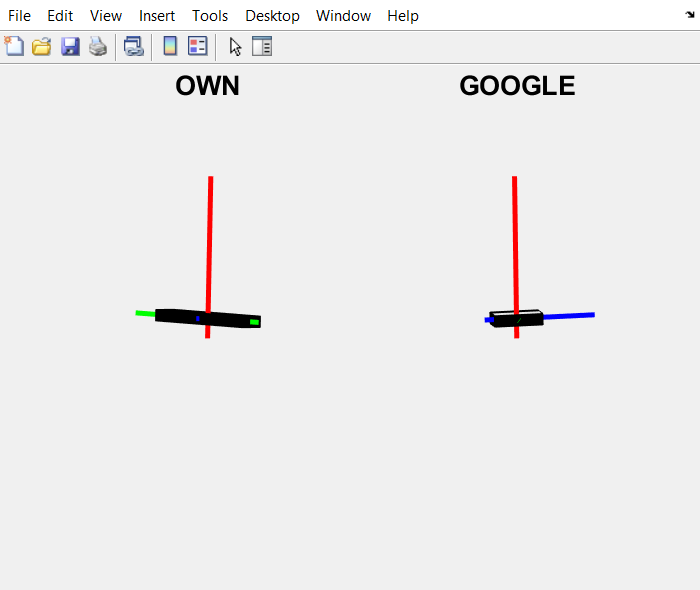
\includegraphics[width=0.6\textwidth]{images/goright.png}
 \caption{Fastly go right}
 \label{fastright}
\end{figure}

During the testing process, we have observed that if the phone does not experience significant acceleration, its own orientation estimate will not drift significantly. However, when the phone undergoes a substantial acceleration that cannot be ignored, such as the force $ f_k^a $, the estimated posture will exhibit significant drift.


\subsection{Task 8}

\begin{figure}[H]
 \centering
 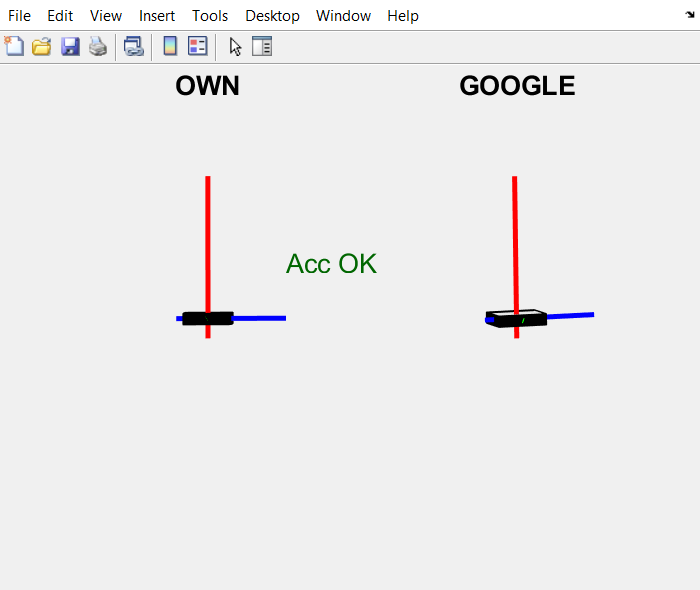
\includegraphics[width=0.6\textwidth]{images/beginwithoutlier.png}
 \caption{20\% range - begin}
 \label{label}
\end{figure}

Set outlier range as 20\%:

\begin{figure}[H]
 \centering
 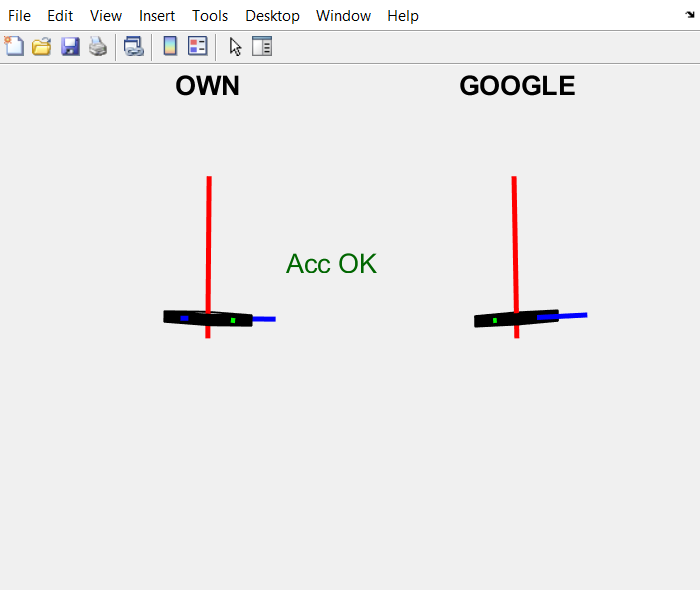
\includegraphics[width=0.6\textwidth]{images/20range.png}
 \caption{20\% range - end}
 \label{label}
\end{figure}

We find that 20\% outlier range is too big that cannot fix the drift, so try to set the range as 10\%:

\begin{figure}[H]
 \centering
 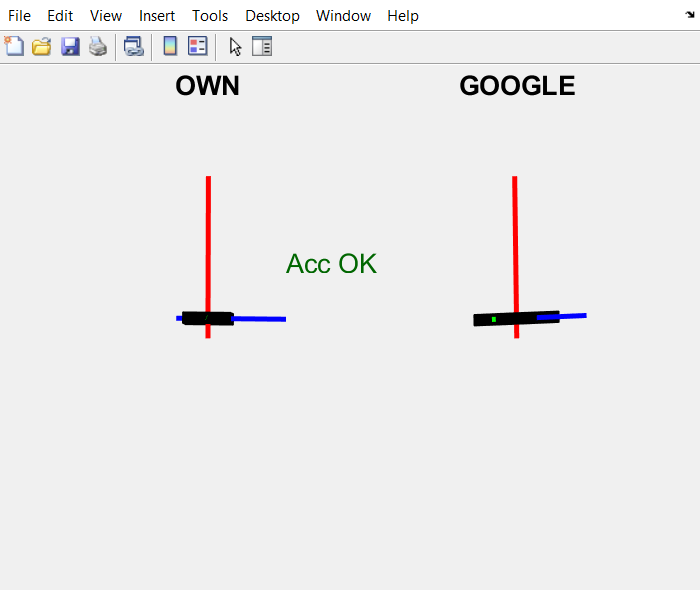
\includegraphics[width=0.6\textwidth]{images/new10begin.png}
 \caption{10\% range - begin}
 \label{label}
\end{figure}

After performing rapid back-and-forth shaking of the phone, it appears that the previous drift issue has been mostly resolved.

\begin{figure}[H]
 \centering
 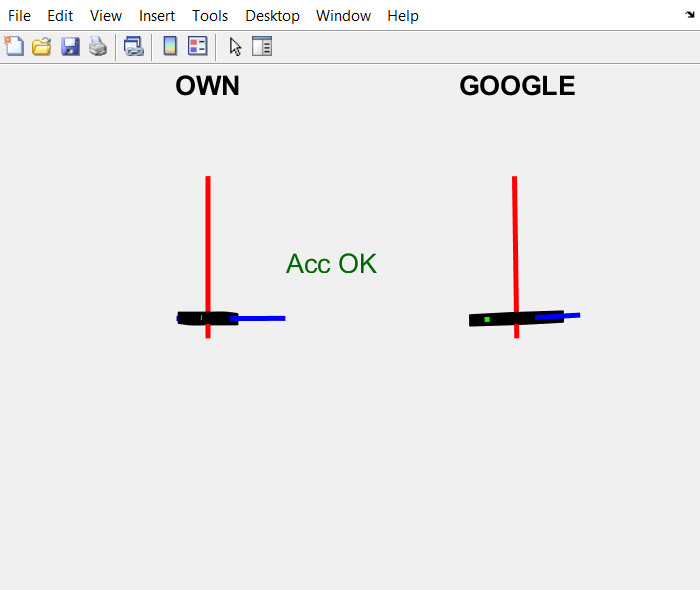
\includegraphics[width=0.6\textwidth]{images/10rangeshake.png}
 \caption{10\% range - end}
 \label{label}
\end{figure}

But after some violent shake, the result still says it is not good:

\begin{figure}[H]
 \centering
 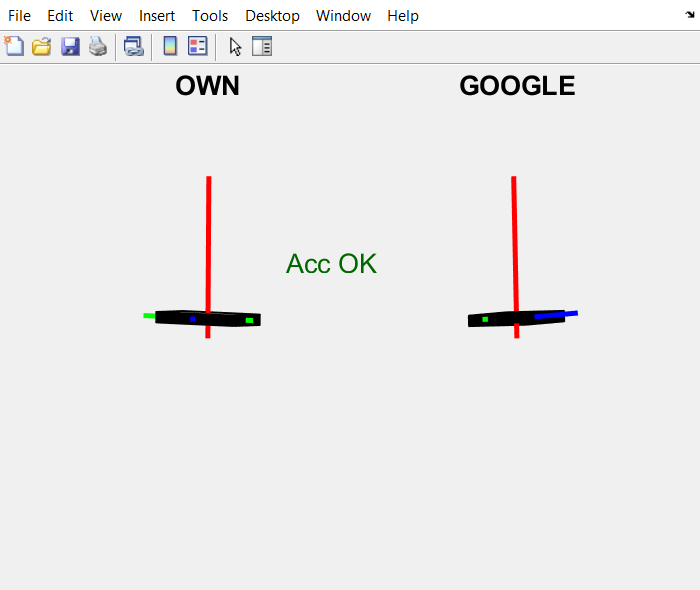
\includegraphics[width=0.6\textwidth]{images/violent10.png}
 \caption{capital}
 \label{label}
\end{figure}


In conclusion, after updating the outlier detection and implementing a rejection threshold, we have observed that the current attitude estimation is able to mitigate the drift issue observed in previous experiments, as long as the acceleration is not excessively high. This outcome aligns with our expectations, as updates falling outside the acceptable range are rejected.

However, we have also noticed that even with the implementation of this simple rejection algorithm, there is still some deviation in the attitude estimation after intense and multi-directional shaking acceleration. This can be attributed to the fact that the orientation estimation algorithm involves integrating accelerometer measurements over time to estimate orientation. Integration introduces cumulative errors, and even small inaccuracies in the accelerometer measurements can result in significant drift over time. Outlier rejection alone may not be sufficient to compensate for these integration errors and maintain accurate orientation estimates. 